\section{Introduction}

%Information access systems, such as recommendation and retrieval algorithms, mediate information exposure and consumption. However, according to an increasing number of studies \cite{DBLP:Diaz} disparities in exposure between retrieved items of such systems may contribute to representational harm\textemdash reinforcing gendered and racialized negative stereotypes\textemdash and allocative harm\textemdash unfair allocation of economic opportunities for historically marginalized groups \cite{Crawford:2017}. 

% 1. The problem
Information retrieval (IR) systems, such as search and recommendation algorithms, mediate exposure and consumption of online information. Traditional IR systems are built on ranking algorithms that maximize utility. However, as recent literature \cite{DBLP:Diaz} \cite{kay} \cite{Singh_2018} suggests, the fairness and biases of ranking algorithms should also be jointly considered. \\

% 2. The body of solutions 
Metrics and methodologies for optimizations are increasingly developed in order to measure and improve fairness in algorithms \cite{DBLP:journals/corr/Burke17aa} \cite{DBLP:journals/corr/abs-2105-05779} \cite{wu}. Precursory research has predominantly focused on the fairness of exposure to users \cite{DBLP:Diaz}. However, as has been argued \cite{DBLP:journals/corr/Burke17aa} \cite{DBLP:journals/corr/abs-2105-05779} group attributes on both consumer and producer sides should be jointly considered to accommodate fairness for all stakeholders. Hence, Wu et al.\cite{wu} introduced a family of six fairness metrics to accommodate a Joint Multisided Exposure fairness perspective. 
% Of particular relevance is the  \textit{expected exposure} metric developed by Diaz. et al
% The paper currently under evaluation contributes to this body of work by (i) formalizing a family of six exposure fairness metric from both consumer and producer perspectives, and (ii) study their decomposition into a relevance and a disparity components. Furthermore, the paper (iii) provides a demonstration of how stochastic ranking policies can be optimized towards spesific JME-fairness goals. \\ 


% 3. Positioning within the related body of work 

%on the \textit{MovieLens1M}- and the \textit{LibraryThing} datasets.

%and conduct additional research in further support of its findings. More specifically, we trained a BERT model, on the same dataset used to train the models used by the authors, and compared with them the achieved fairness measured by their proposed metrics. Additionally, we performed metric analysis using a different dataset to verify that the same patterns apply. 

%In this paper, the authors Wu et al.\cite{wu} extend the proposed framework of Diaz et al. \cite{DBLP:Diaz} by providing a formal formulation of joint multisided exposure (JME) fairness metrics, which provide a broader new range of fairness concerns which they claim are necessary for the development of fair recommendation algorithms.

\section{Scope of reproducibility}
\label{sec:scope_reproducibility}

In this report, we evaluate the reproducibility of the proposed JME-fairness metric properties. The metric family extends upon the concept of expected exposure as the expectation of a user browsing model provided a stochastic ranking policy \cite{DBLP:Diaz}. If the reader is unfamiliar with the aforementioned concepts we invite them to consult section 3.1. In our understanding, the main claims of the original paper can be summarized as follows:

\begin{enumerate} %[label = {--}]
    \item \label{itm: claim1} Stochasticity impacts the JME-fairness metrics and their corresponding disparity and relevance components, in the sense that there exists a disparity-relevance trade-off for each JME-fairness metric.
    \item \label{itm: claim2} Each JME-fairness metric quantifies a different notion of unfairness: a system that performs well on one fairness dimension can be suboptimal for another.
    \item \label{itm: claim3} Recommender systems can be optimized towards a specific fairness goal, based on different combinations of JME-fairness metrics
\end{enumerate}


%The subsequent work aimed to verify the original paper's main claims, which states that 
%present our  we aimed to verify the claims of the paper by performing a reproduction study. 
%In addition, we contributed to the research by studying the framework's application to the neural ranking model BERT

%Unlike earlier research in learning-to-rank with deterministic ranking policies \cite{TieYan2009}, the authors of this paper use stochastic ranking policies to guarantee a more fair distribution of information content. They formalize a family of exposure fairness metrics with group attributes on both the consumer and producer sides, while also providing a metrics analysis. Additionally, the paper proposes a way  to optimize recommendation systems for multiple JME-fairness metrics. In our reproducibility study, we investigate the following research claims:

%The authors of this paper aim to prove the usefulness of the proposed JME-fairness metrics by considering their application in the information retrieval task of recommendation systems. Unlike earlier works in learning-to-rank for IR \textcolor{red}{30}, which are based on deterministic ranking policies, the authors use stochastic ranking policies to ensure fairer exposure of information content \textcolor{red}{17,52,62}. Randomization in ranking was introduced by Pandley et al \textcolor{red}{41} and since then several works have employed it to achieve different goals \textcolor{red}{25,26,40,4,46,47}. Additionally, the paper aims to demonstrate how stochastic ranking policies for recommendation can be optimized towards JME-fairness.
%\\ Τhe authors decompose each metric into three components: a disparity and a relevance component as well as a system-independent constant. To test the impact of stochasticity, they visualise how different levels of stochasticity influence the different metrics and their corresponding components. Additionally, cross-metric analysis is conducted to provide understanding on how a recommender system optimized for one JME-fairness metric may influence other measures.
%The results of the experiments can be summarized in three main claims:



%\jdcomment{To organizers: I asked my students to connect the main claims and the experiments that supported them. For example, in this list above they could have ``Claim 1, which is supported by Experiment 1 in Figure 1.'' The benefit was that this caused the students to think about what their experiments were showing (as opposed to blindly rerunning each experiment and not considering how it fit into the overall story), but honestly it seemed hard for the students to understand what I was asking for.}

\section{Methodology}
%Parts of the original implementation of the JME Fairness metrics and analysis is published \cite{Wugit2022}, but the experiments are not.  
In the subsequent section, we provide fundamental concepts and definitions that were adopted by Wu et al. \cite{wu} and information on the design of our experiments.

\subsection{Browsing models, stochastic ranking and exposure}
\label{sec:model_description}
User browsing models estimate the probability of exposure of an item \textit{d} in a retrieved ranked list of items \textit{$\sigma$}. The browsing model used in this paper is the rank-biased precision (RBP) metric \cite{Moffat2008} which presumes that the probability of the exposure event \textit{$\epsilon$} for \textit{d} depends only on its rank $\rho_{d, \sigma}$ in a retrieved ranked list \textit{$\sigma$} and decreases exponentially as:
\begin{center}
    $p(\epsilon|d, \pi_{u}) = \gamma^{(\rho_{d, \sigma}-1)}$
\end{center}
The patience factor $\gamma$ determines how far down the ranking the user is likely to explore. \\
 
A stochastic ranking policy $\pi$ is a probability distribution that covers all item arrangements in the collection \cite{DBLP:Diaz}. Given such a policy $\pi_u$ conditioned on user $ u\in \mathcal{U}$, the expected value of the probability that an item $d\in \mathcal{D}$ is exposed to the user is:

\begin{center}
   \begin{equation}\label{eq1}
       p(\epsilon|d, \pi{u}) = \mathbb{E}_{\sigma \sim \pi_u}[p(\epsilon|d, \sigma)]
   \end{equation} 
\end{center}
The authors refer to E $\in \mathbb{R}^{|\mathcal{U}|x|\mathcal{D}|}$ as the expected exposure matrix, such that E$_{ij} = p(\epsilon|\mathcal{D}_{j}, \pi_{\mathcal{U}_{i}})$. The three expected exposure matrices E defined by the authors are \textit{system exposure  E}, the expected exposure corresponding to a stochastic ranking policy $\pi$ as determined by a retrieval system; \textit{target exposure E$^*$}, the expected exposure corresponding to an ideal stochastic ranking policy $\pi^*$ (e.g., the equal expected exposure principle \cite{DBLP:Diaz} ); \textit{random exposure E$^\sim$}, the expected exposure corresponding to a stochastic ranking policy $\pi^\sim$ defined by a uniformly random distribution over all item permutations.

\subsection{Metric definitions, decomposition and method for metric analysis}
\label{sec:metrics}
The formal mathematical definitions for the metrics proposed in the paper can be seen in Table \ref{metric_def} \cite{wu}. Each of the metrics represents a different fairness concern measuring the deviation between system exposure and target (ideal) exposure. The first dimension of each metric refers to the users while the second refers to the items. The letters ``I'', ``G'' and ``A'' correspond respectively to individual users or items, groups of individuals or items, and all individuals. For all six metrics, to have a fairer recommendation system, lower values are more desirable. 

\begin{table}
\centering
\begin{tabular}{l}
\hline
\textbf{Metric} \\
\hline
\textbf{II-F} = $\frac{1}{|D|} \frac{1}{|U|} \sum\limits_{j=1}^{|D|} \sum\limits_{i=1}^{|U|} (E_{ij} - E^*_{ij})^2$  \\
\textbf{IG-F} = $\frac{1}{|G_d|} \frac{1}{|U|} \sum\limits_{D \in G_d} \sum\limits_{i=1}^{|U|} (\sum\limits_{j=1}^{|D|} p(D_j|D)(E_{ij} - E^*_{ij}))^2$ \\
\textbf{GI-F} = $\frac{1}{|D|} \frac{1}{|G_u|} \sum\limits_{j=1}^{|D|} \sum\limits_{U \in G_u} (\sum\limits_{i=1}^{|U|} p(U_i|U)(E_{ij} - E^*_{ij}))^2$ \\
\textbf{GG-F} = $\frac{1}{|G_d|} \frac{1}{|G_u|} \sum\limits_{D \in G_d} \sum\limits_{U \in G_u} (\sum\limits_{j=1}^{|D|} \sum\limits_{i=1}^{|U|} p(D_j|D) p(U_i|U)(E_{ij} - E^*_{ij}))^2$ \\
\textbf{AI-F} = $\sum\limits_{j=1}^{|D|} (\sum\limits_{i=1}^{|U|} p(U_i)(E_{ij} - E^*_{ij}))^2$ \\
\textbf{AG-F} = $\frac{1}{|G_d|}\sum\limits_{D \in G_d}(\sum\limits_{j=1}^{|D|} \sum\limits_{i=1}^{|U|} p(D_j|D)p(U_i)(E_{ij} - E^*_{ij}))^2$ \\
\hline
\end{tabular}
\caption{\label{metric_def}
The formal mathematical definition of the JME-fairness metrics
}
\vspace{-5mm}
\end{table}

Each proposed metric can be decomposed into three components: a disparity and a relevance component and a system-independent constant. This allows one to study the trade-off between disparity and relevance, while different degrees of stochasticity are introduced into the model. The use of a static ranking model with all relevant items at the top maximizes relevance and a fully stochastic model minimizes disparity. The decomposition for the JME-fairness metrics can be seen in Appendix \ref{decomposed_metrics}.
\\ \\
A method to generate stochastic ranking policies with varying levels of stochasticity is introduced, in order to examine their ability to distribute item exposure. The Plackett-Luce (PL) model~\cite{Luce59}~\cite{plackett} is utilized to produce multiple rankings by sampling from the estimated relevance scores of items for a user, given a deterministic ranker. The model is based on Luce's axiom that the probability of choosing one item over another does not depend on the set of items from which the choice is made \cite{Luce59} \cite{Luce1977TheCA} and creates a ranking by repeatedly selecting items without replacement from the collection with probability distribution defined as: 
\begin{center}
$p(d|u) = \frac{exp(Y_{d,u}/\beta)}{\sum_{d' \in D} exp(Y_{d',u}/\beta)}$
\end{center}
The parameter $\beta$ controls the level of stochasticity of the ranking model. A higher value corresponds to more stochasticity, while a lower value indicates a more deterministic ranking policy. $Y_{d,u}$ represents the relevance score for item d for user u, estimated by the deterministic ranker.

\subsection{Datasets}
The original work conducts its primary experiments on the MovieLens1M \cite{movielens1m} dataset comprised of movie reviews. In addition, the MovieLens100k dataset is considered for the optimization task. However, the current work disregards the MovieLens100k dataset as we were not able to reproduce the optimization experiment. To conduct further experimentation regarding the claims within the original paper, we also consider the LibraryThing \cite{inproceedings}\cite{inproceedings2} dataset comprised of book reviews. 
\\ \\
\textbf{MovieLens1M (ml-1m)} consists of 1,000,209 numerical ratings ranging from 1-5. The reviews are supplied by 6,040 MovieLens users on 3,706 movies. The available metadata for the users includes 2 gender groups, 7 age groups, 21 occupation groups, and zip codes. The metadata for the movies comprises 19 genre groups (including unknown). Each user in the dataset has written at least 20 reviews. 
\\ \\
\textbf{LibraryThing (lt)} Due to computational limitations, we extract a subset of the LibraryThing dataset comprised of 702,522 reviews provided by 12,976 LibraryThing users on 325,075 books. The selection is made so that each user has written at least 20 reviews and each item is reviewed at least 3 times. 

\subsection{Hyperparameters}
In order to reproduce the results of the original paper we set the hyperparameters equal to the default parameters found in the original codebase. The values used to perform metric analysis on both datasets are listed in Table \ref{hyp}.

\begin{table}[ht]
\centering
\begin{tabular}{ |p{2.2cm}|p{0.5cm}|p{4.5cm}|p{3.3cm}| }
\hline
\hfil\textbf{Dataset} & \hfil$\mathbf{\gamma}$ & \textbf{User Group Attributes} & \textbf{Item Group Attribute}\\ \hline
\textbf{MovieLens1M}&0.8& gender, age, occupation & movie genre\\ \hline
\textbf{LibraryThing}& 0.8& helpfulness of users' ratings & engagement rate\\
\hline
\end{tabular}
\caption{\label{hyp}
Hyperparameter values for the metric analysis experiments}
\end{table}

In particular, we introduce 8 degrees of stochasticity with $\beta =$\{8,4,3,2,1,0.5,0.25,0.125,ST\}, where ST refers to a fully static deterministic model. While the MovieLens dataset supplies group attributes such as age, gender, and occupation, the LibraryThing dataset only provides an evaluation rate of the helpfulness of each user's ratings and a comment per movie. As such, we construct an 'engagement' group attribute for each item derived as the average length of its received comments. Furthermore, the user attribute is built by calculating the average number of helpfulness votes received by each user.\\

For the Bert4Rec model, we initialize the embedding dimension for the hidden layers to 128, with the length of BERT embeddings being at a maximum of 100 items. The learning rate is set to 0.001.

\subsection{Experimental setup and code}
\subsubsection{Code} An open-source implementation of code associated with the original paper was published by the authors on \href{https://github.com/haolun-wu/JMEFairness}{GitHub}. Unfortunately, we experienced several conflicts when we attempted to deploy the code. In particular, no code was provided to run the baseline experiments of the original paper, the hyperparameters used in each experiment were not specified and dependencies were not always clarified. Due to insufficient compartmentalization and documentation, the code was generally hard to understand. A full account of the issues we encountered is provided in Appendix \ref{code_issues}. In order to ease future research and extensions utilizing the code, we provide a restructured codebase with a higher degree of documentation, supplied with additional postprocessing and configuration tools for the experiments.

\subsubsection{Pipeline} 
Identical to the original pipeline we employ the RBP user browsing model. Stochastic ranking policies with stochasticity $\beta$ are generated over a set of trained deterministic ranking models for the MovieLens1M and the LibraryThing dataset. The pre-trained models are supplied by Valcarce et al. \cite{Valcarce2018} and were made available through \href{https://github.com/dvalcarce/evalMetrics}{GitHub}. The fairness metrics are then computed utilizing the expected exposure of equation \ref{eq1}, the formal fairness definitions of section \ref{sec:metrics}, and their decomposition as described in section \ref{sec:metrics}. 

\subsubsection{Claim 1} In order to verify claim \ref{itm: claim1} we estimate the fairness metrics across 8 different levels of stochasticity $\beta$ and reproduce Figures \ref{fig: og_fig2} and \ref{fig: og_fig3} as well as Table \ref{original_auc}, included from the original paper. 
While the authors mentioned that they applied min-max normalization, they did however not state how the normalization was applied. As such, we made the following assumptions based on the min-max values of the original figures: to obtain Figure \ref{fig: og_fig2}, we perform a min-max normalization over the estimated metrics for each metric dimension and for each component separately, across all stochasticity values. We perform the same analysis across all 21 pre-trained ranking models available in the repository. To obtain Figure \ref{dr_tradeoff} we perform a normalization per metric component across the models \textit{BPRMF, LDA, PureSVD, SLIM} and \textit{WRMF}. With regards to Table \ref{original_auc}, the authors do not clearly state how the area under the curve (AUC) is calculated. Initially, we did this using the trapezoidal rule. However, after consulting the authors it was made clear that the AUC was calculated for each curve only up until the disparity value which corresponds to the smallest stochastic value across all models. We reproduce Table \ref{auc} to quantify the disparity-relevance tradeoff across all five models and calculate the average relative difference between our results and their results. 

\subsubsection{Claim 2} In order to verify claim \ref{itm: claim2} we compute the Kendall rank correlation \cite{kendall_rank}  between the different metrics and their relevance and disparity components across all six proposed fairness dimensions on the pre-trained models. The authors of the original paper state that they evaluate 15 different pre-trained deterministic rankers on the MovieLens1M dataset, for 8 different levels of stochasticity. However, as they do not specify which models are used and the codebase provides 21 pre-trained models, we perform the analysis over all of them. The analysis is performed using gender and age as user-side group attributes. 
%\textcolor{red}{Following sentence refers to an extension we are not sure we will incorporate: heatmaps on libthing} We reproduce the analysis on the LibraryThing dataset using the respective constructed attributes, to assess whether the relationship between the metrics is independent of the input data. 

\subsubsection{Claim 3} The authors provided no codebase for the third claim, but they did provide a general algorithm and proposition for a JME-fairness loss that could be used in a training situation. From there, we attempted to train a BPRMF model with the proposed loss. As we were not able to reproduce their results, its methodology is not elaborated on in this report. However, we advise the curious reader to consult section 6 of the original paper for further information. 

\subsubsection{Beyond the paper: Experiment I} 
NN-based approaches to IR have witnessed an explosive growth in recent years \cite{kenter2018} \cite{mitra2017neural} \cite{Onal2018NeuralIR}, yielding state-of-the-art ranking methodologies such as the Bert4Rec model \cite{Sun:2019}. As such, it is becoming increasingly important to develop scalable fairness frameworks that can mediate multisided exposure fairness for all stakeholders. We extend upon the work by Wu et al. by demonstrating the application of the JME-fairness metric to a neural model and evaluating if their claims are still valid. \\

We train a Bert4Rec model from scratch and apply it to both the ml-1m and the lt datasets. Bert4Rec is a recommender that is a combination of two SOTA models: the BERT language model and SASRec recommender system. Using the bidirectional ability of BERT on top of a sequential recommender allows the model to capture more complex user behaviors. For the BERT4Rec model \cite{Sun:2019}, we adopt a PyTorch implementation available from the TorchRec library \cite{Sungit2019}. Both datasets are split into a training, validation, and test set based on leave-one-out, where the second-last and last reviewed items of a user are reserved for validation and testing respectively. We train 10 epochs on the Movielens dataset and run the JME metrics on the obtained predictions as in the original paper, including different levels of stochasticity. However, even after our modification, the LibraryThing dataset still exhibits high sparsity. Therefore, achieving 10 epochs on this particular dataset is not computationally feasible with our current resources. 

\subsubsection{Beyond the paper: Experiment II} 
In the original experiments, age and gender are used as group attributes on the user side, we perform the analysis with the Kendall rank correlation with a different attribute: \textit{occupation}. The attributes used originally present very few groups which could be the cause for the high correlation between group-related metrics (GG-F AG-F) in Figure \ref{kendall}. We perform this analysis to investigate whether the same trends are consistent when considering more groups. 

\subsubsection{Beyond the paper: Experiment III}
To assess the validity of the author's choice for the hyperparameter value $gamma=(0.8)$, we conducted an additional parametersweep through assigning different values for $\gamma = [0.01, 0.2, 0.4, 0.6, 0.8, 0.9]$ and analyzing the behavior of the JME fairness metric on a BPRMF model.
\\
All experiments presented in this document can be reproduced by using the code provided in this \href{https://github.com/OlineRanum/FACT.git}{GitHub} repository. In the \href{https://github.com/OlineRanum/FACT#readme}{README} section we provide instructions on how to obtain the results for the different experiments. 

\subsection{Computational requirements}
The experiments are conducted on a local machine with the GPU model GeForce RTX 3070 equipped. The total calculated computational costs for running the metrics, with and without a stochastic policy, can be seen in Appendix \ref{computation_costs}.

\section{Results}
\label{sec:results}
In this section, we present the results of our reproducibility study and of our extended research.
We include the results of the original paper in Appendix \ref{og_results} for the readers' convenience and completion.

\subsection{Results reproducing original paper}
\subsubsection{Result 1} Our reproduction of the JME-fairness stochasticity impact study is presented in Figure \ref{fig2}, the disparity-relevance trade-off is presented in Figure \ref{dr_tradeoff} and the AUC estimates in Table \ref{auc}. Larger stochasticity implies a more fair system, governed by small relevance and disparity. At a qualitative level, we successfully reproduced the trends observed in Figure \ref{fig: og_fig2} of the original paper. However, when considering Figure \ref{dr_tradeoff} and Table \ref{auc} we observe that the relationships between the performance of the models deviate from the relationships found in the original paper. For instance, across the II-dimension, the trends of SLIM and LDA are flipped with respect to Wu et al. When considering the AUC we observe the same deviations in trends from the original paper and find that on average, across all models, our results deviate with $25\pm6\%$. 

\begin{figure}[ht]
    \centering
    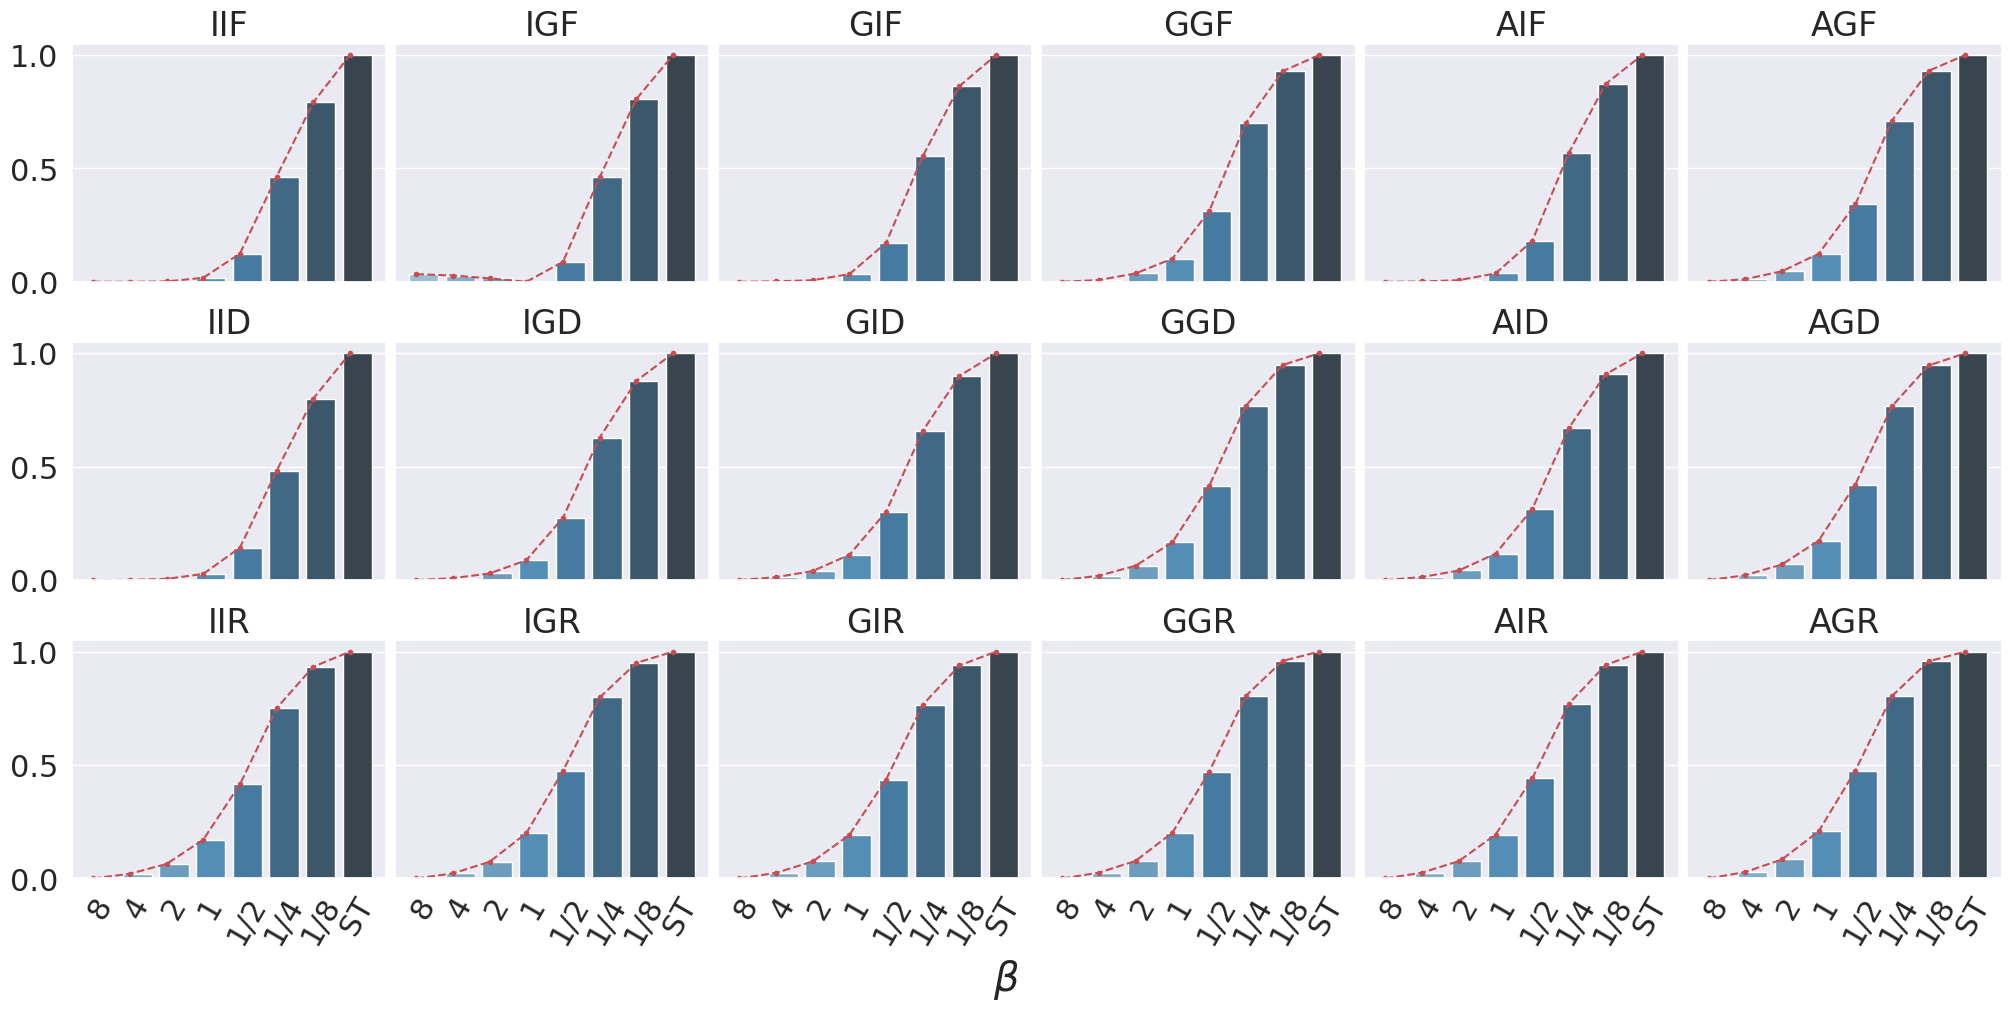
\includegraphics[width=\columnwidth]{Figures/Figure_2.png}
    \caption{Behaviour of JME-fairness metrics for a stochastic ranking policy. Bars are produced by randomizing the BPRMF model using the Plackett-Luce model on MovieLens1M dataset. First, second and third rows correspond respectively to the impact of different stochasticity on the overall fairness, disparity, and relevance components. The x-axis shows the values of $\beta$, where a larger value indicates more randomization}
    \label{fig2}
%\vspace{-4mm}
\end{figure}
\begin{figure}[ht]
    \centering
    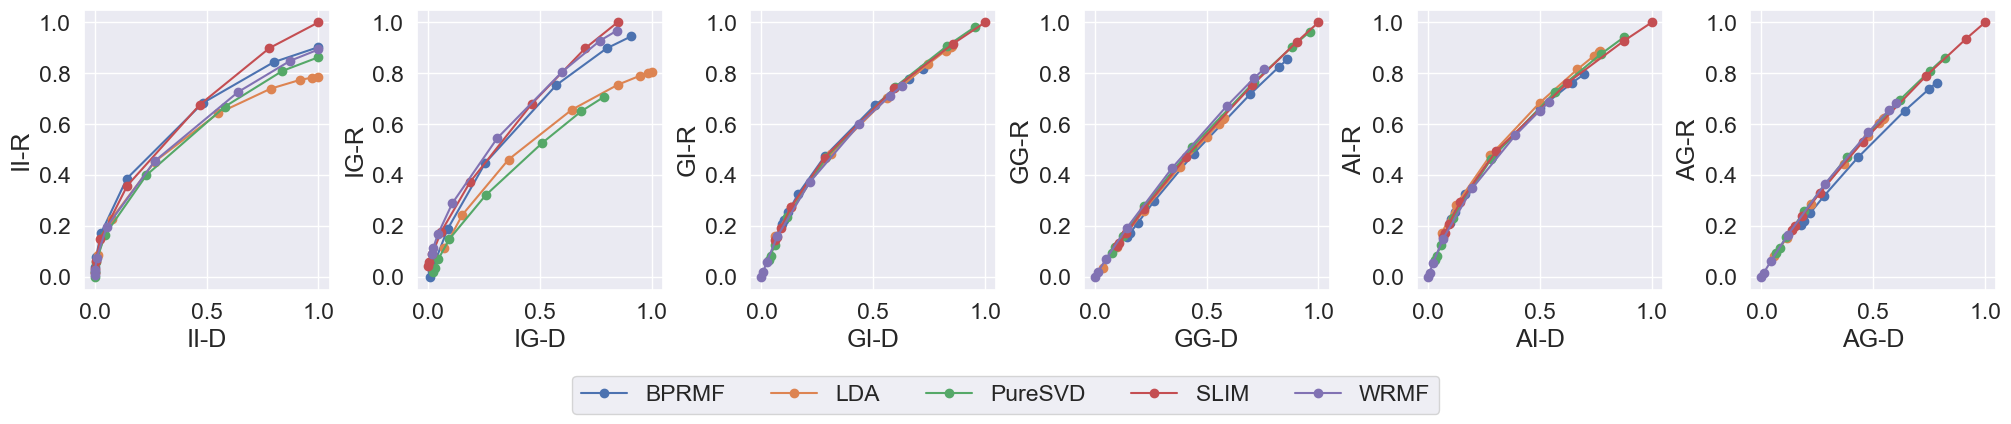
\includegraphics[width=\columnwidth]{Figures/Figure_3_Age.png}
    \caption{Disparity-relevance trade-off curves across six fairness dimensions with 8 levels of stochasticity for 5  recommendation models}.
    \label{dr_tradeoff}
\vspace{-4mm}
\end{figure}
\begin{table}[ht]
    \centering
    \begin{tabular}{lllllllc}
        \hline
        \textbf{Model} & \textbf{II} & \textbf{IG} & \textbf{GI} & \textbf{GG} & \textbf{AI} & \textbf{AG} & \textbf{Avg. rel. diff.}\\ 
        \hline
        BPRMF  &  \ \underline{0.6336} & \underline{0.437} & 0.1949 &  0.2487  &  0.1879  & 0.0869 & 0.26 \\
        LDA  &  0.5567 & 0.2448  & 0.2305  &  0.1877  & \underline{0.2007}   & \underline{0.1799}  & 0.28\\ 
        PureSVD  &  0.5691  &  0.3239  &  \underline{0.2615}  & \underline{0.2896}  & 0.0712  &  0.0909  & 0.30\\ 
        SLIM  &  \textbf{0.6540}  &  0.3757  &  0.2591  &  0.2739  &  0.0799  &  0.1145 & 0.27 \\ 
        WRMF  &  0.5901  &  \textbf{0.5171}  &  \textbf{0.2826} &  \textbf{0.334}  &  \textbf{0.2194}   &  \textbf{0.2219}  & 0.13\\ 
        Bert4Rec & 0.7325 & 0.6331 & 0.7495 &  0.6229  & 0.7626  & 0.6026 &\\ 
        \hline
    \end{tabular}
    \caption{\label{auc}
    The AUC of the disparity-relevance trade-off curves for 5 pre-trained models and Bert4Rec across 6 fairness dimensions. Highest and second highest value of each column is marked bold and underlined. Rightmost column shows the average relative difference with respect to the AUC calculated with our method.}
    \vspace{-4mm}
\end{table}
\begin{figure}[ht]
    \centering
    \includegraphics[width=0.32\textwidth]{Figures/Figure_4_Age_0.png}
    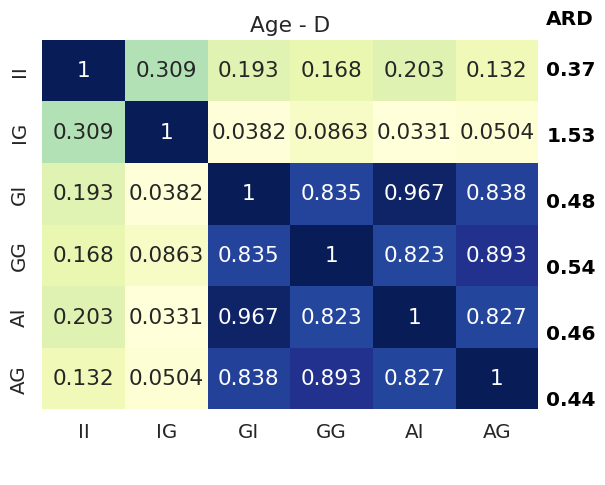
\includegraphics[width=0.32\textwidth]{Figures/Figure_4_Age_1.png} \includegraphics[width=0.32\textwidth]{Figures/Figure_4_Age_2.png}
    \\
    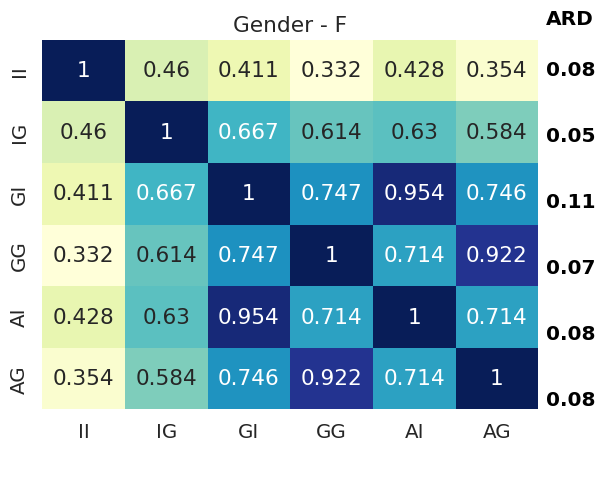
\includegraphics[width=0.32\textwidth]{Figures/Figure_4_Gender_0.png}  \includegraphics[width=0.32\textwidth]{Figures/Figure_4_Gender_1.png}  \includegraphics[width=0.32\textwidth]{Figures/Figure_4_Gender_2.png} 
    \caption{The Kendall rank correlation between the six JMEF metrics and their two components. The first, and second rows correspond to age, and gender user attributes. From the left to the right column, we respectively find the heatmaps for the fairness, disparity, and relevance components.}
    \label{kendall}
\end{figure}

\subsubsection{Result 2} 
To verify claim \ref{itm: claim2} we reproduce the Kendall rank correlations and present them in Figure \ref{kendall}. We observe that the trends of our results follow similar patterns as the ones observed by Wu et al. Our cross-metric analysis demonstrates a relatively low correlation between II-F and all other metrics. Additionally, for both group attributes it can be seen that there is a high correlation between the GG and AG metric, due to the low number of groups. 

\subsubsection{Result 3} 
In our attempts to optimize a BPRMF model with the fairness loss we encounter vanishing gradient problems, and we are not currently able to make the loss converge. As such, we are not able to reproduce claim \ref{itm: claim3}.

\newpage
\subsection{Results beyond original paper}
\begin{figure}[ht]
    \centering
    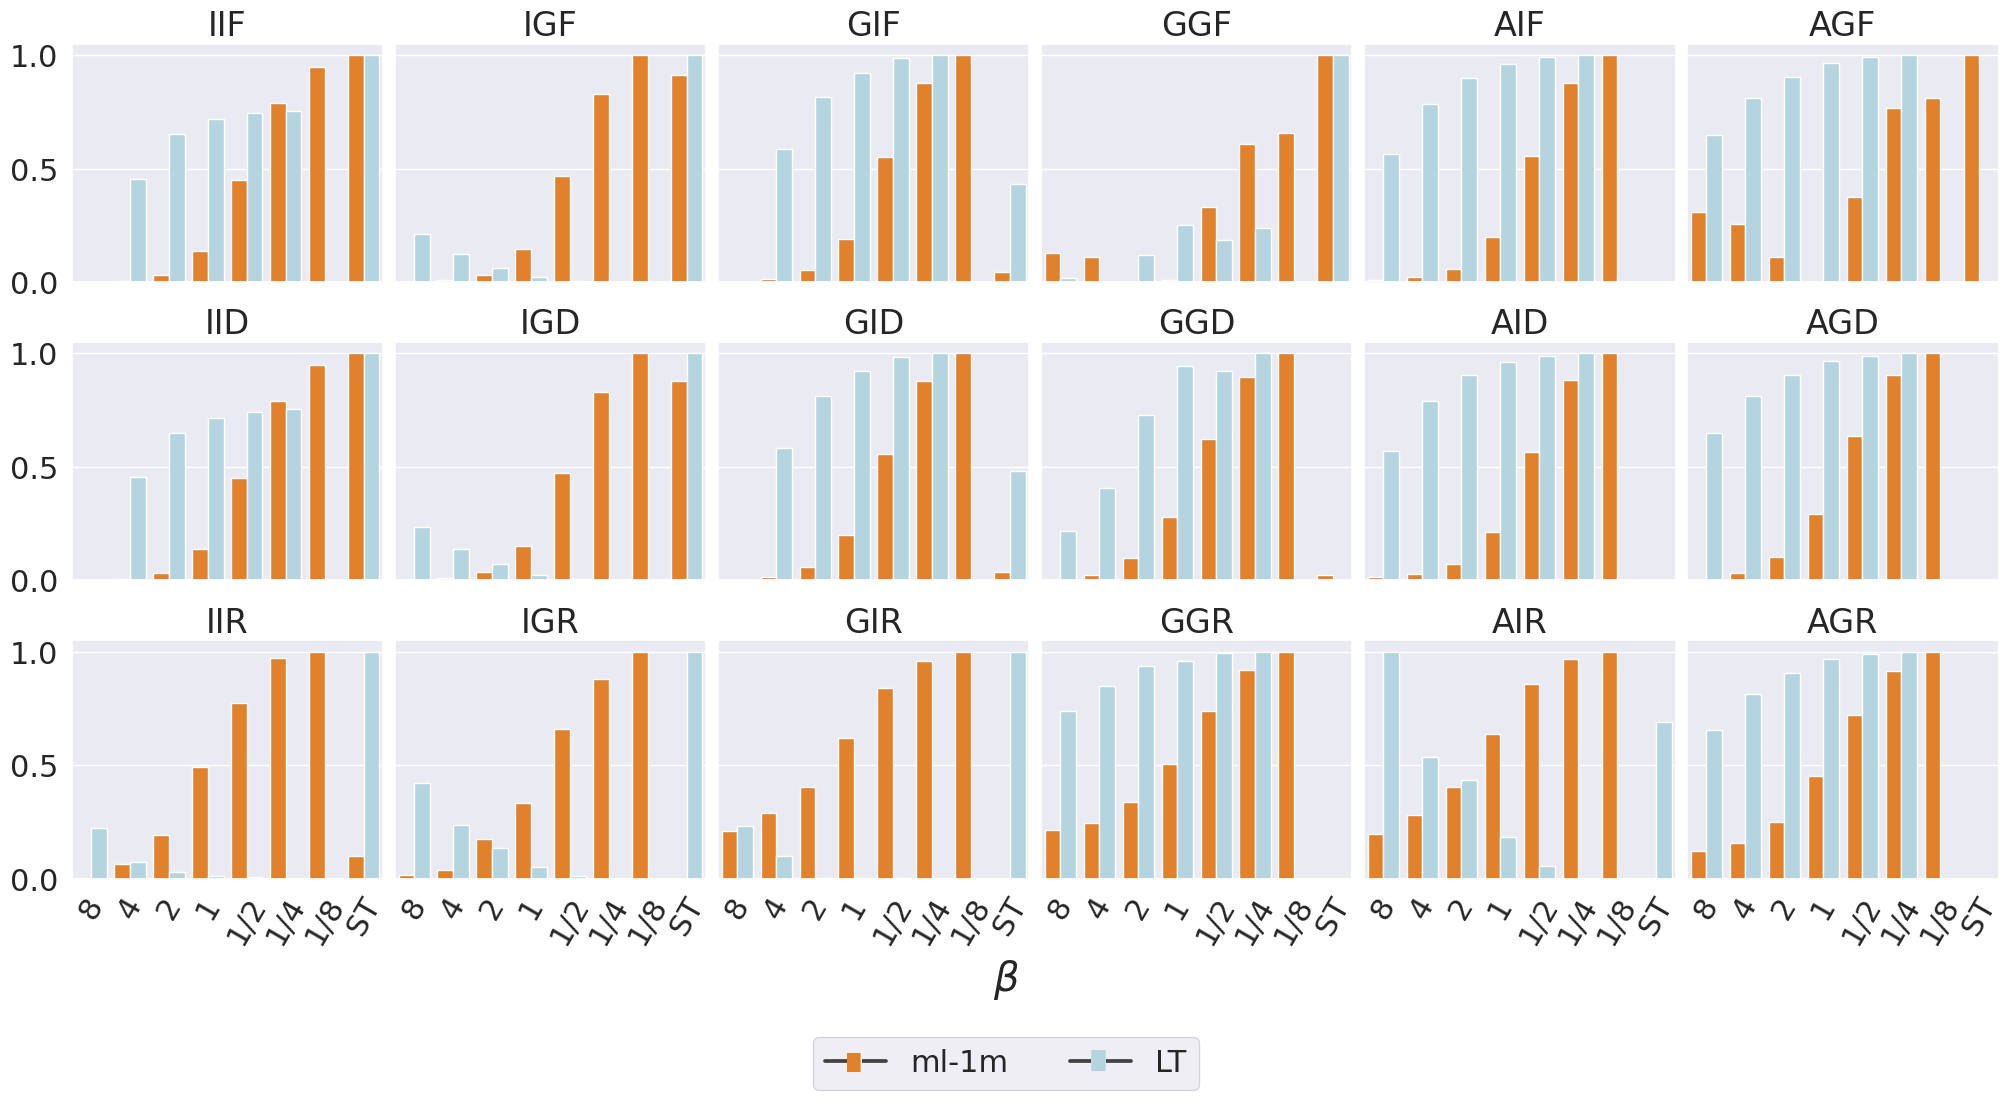
\includegraphics[width=\columnwidth]{Figures/Figure_5.png}
    \caption{Comparison of Bert4Rec metrics' and disparity and relevance components on MovieLens1M and LibraryThing}
    \label{bert_metrics}
\end{figure}
\subsubsection{Additional Result 1}
The behavioral results of the JME metrics on a neural model can be observed in Figure \ref{bert_metrics}, and the AUC of the ml-1m dataset is presented in Table \ref{auc}. For the ml-1m dataset, we observe that the metrics generally decrease as $\beta$ increases. From this, we confirm the presence of a disparity-relevance trade-off, since the stochastic ranking policy still fails to achieve low disparity and high relevance concurrently. In addition, the AUC indicates that the trade-off is generally better than the ones of the deterministic models. Noticeably, the static ranking policy tends to show poor values compared to its stochastic variant when we consider user groupings. As aforementioned, we did not succeed in producing a complete model trained on the LibraryThing dataset due to computational and time limitations. Nonetheless, we chose to include a preliminary evaluation on the 5th epoch in Figure \ref{bert_metrics} as a demonstration of the metrics on a weak recommender system.

\subsubsection{Additional Result 2}
The Kendall rank correlation for the occupation groups can be observed in Appendix \ref{occupation_kendall}. Although the calculation is computed across a larger number of groups, the correlation between GG-F and AG-F is still high, leading to the conclusion that even the considered 21 occupational groups are too few to lessen their correlation. The results are presented in the Appendix as they are trivial. 

\subsubsection{Additional Result 3}
The results of our parametersweep can be found in the Appendix \ref{paramter_sweep}. Considering the definition of $\gamma$ as the patience factor, it describes the probability of an user progressing to the next item in the ranked list \cite{Moffat2008}. In our case, a low $\gamma$ value would indicate a smaller set of items being exposed to users, resulting in lower fairness due to limited diversification. From our results, the behavior of the JME fairness coincides with this assumption, assigning higher fairnesses to higher patience factors, whereas a lower values are scored lower. As for why $0.8$ is specifically chosen by the authors can be derived from the work of A. Moffat and J. Zobel(2008)\cite{Moffat2008}, where values between $0.5$ and $0.8$ have been assessed to be the most stable for rank-biased precision. 

\section{Discussion}
%Give your judgement on if your experimental results support the claims of the paper. Discuss the strengths and weaknesses of your approach - perhaps you didn't have time to run all the experiments, or perhaps you did additional experiments that further strengthened the claims in the paper.
In this work, we found that our reproduction study could provide support for two out of three claims, with minor numerical discrepancies. The inconsistencies could be due to the use of different hyperparameters, for instance, the seed as these were not explicitly clarified in the original paper. In Figure \ref{kendall} we observed varying degrees of numerical deviations. A plausible reason is that we utilized different data in taking into consideration all 21 models. Regarding the experiments on the neural model, we observed behavior across several dimensions deviating from the expected trend posed by the deterministic rankers. This is presumably due to insufficient training but does not exclude the possibility of flaws in the model's inherent properties, which we recommend to be further investigated. It would demonstrate that even if our model achieves favorable results on standard evaluation scores, additional analyses are to be considered with regard to the model's task.  

%Throughout this study, we have conducted many experiments to reproduce the main results presented in the original paper. The results of our experiments provide support for their claims, although with some minor numerical discrepancies. 
%Some of them are found in the disparity-relevance curves shown in Figure \ref{dr_tradeoff}, this could be due to the use of a different seed from the original authors during their implementation, or the use of different hyperparameters, as they were not specified in the original paper and we conducted the experiments with the default values.
%Additionally, for the reproducibility of claim \ref{itm: claim2}, the results obtained from the experimentation differ slightly due to the use of different models from the ones used by the authors.
%As regards the experiments beyond the original paper, the lacking performance on the MoviLens1M dataset towards fairness, shown in Figure \ref{bert_metrics}, is 
% need to write a discussion about occupational group heatmap, just writing down some notes
%As both for age and gender, there are very few groups it is expected to find a higher correlation among GG and AG metrics. 
%The opposite is true in the standard settings of the experiment where age and gender are used, as they are both small groups. However, in the dataset, there are 21 occupational groups. Therefore the number of groups might not be the only explanation for this high correlation.

\subsection{What was easy}
The explanation of each of the proposed JME-fairness metrics was very well-written and easy to follow even for someone with no previous background in the field of fairness in AI. Additionally, the relationship between the metrics and their decomposition was clearly explained and accompanied by examples allowing for comprehension even without very advanced mathematical knowledge.

\subsection{What was difficult}
The code provided in the original repository was complex and hard to interpret as it was lacking adequate documentation. Large parts of the code required to recreate the original experiments were missing. Additionally, no environment was provided thus, we had to make some assumptions about the requirements to run the experiments and create one.
%There were also some bugs in the code regarding the separation of users into age groups that needed to be rewritten.
Finally, as there was no publicly available code to optimize for JME-fairness, deeper knowledge regarding the mathematical concepts behind the algorithm was required to implement it from scratch.

\subsection{Communication with original authors}
We reached out to the authors to get clarifications on several matters. We asked for clarifications regarding the calculation of the AUC of Table \ref{auc}, as the methods that seemed intuitively correct produced different results from the ones in the original paper. Furthermore, we requested more details regarding the setup for the experiments for claim \ref{itm: claim3} as they voluntarily did not include their implementation in their repository. They provided us with their way to calculate the AUC, with some indications on the pipeline used to support claim \ref{itm: claim3} and with a possibly helpful external paper.

\newpage